\documentclass[12pt,a4paper]{article}
\usepackage[a4paper,margin=1in,headheight=15pt]{geometry}
\usepackage[T1]{fontenc}
\usepackage[utf8]{inputenc}
\usepackage{mathptmx}
\usepackage{microtype}
\usepackage{setspace}
\usepackage{amsmath,amssymb,mathtools}
\usepackage{booktabs,longtable,array,tabularx,multirow}
\usepackage[table]{xcolor}
\usepackage{graphicx}
\usepackage{caption}
\usepackage{float}
\usepackage{enumitem}
\usepackage{fancyhdr}
\usepackage{titlesec}
\usepackage{tocloft}
\usepackage{url,xurl,hyperref}
\usepackage{tikz}
\usepackage{pgfplots}
\usepackage{pgfplotstable}
\usetikzlibrary{arrows.meta,positioning,shapes.geometric,fit}
\pgfplotsset{compat=1.18}

\definecolor{MainBlue}{HTML}{1F4E79}
\definecolor{LightBlue}{HTML}{DCE6F1}
\definecolor{SoftGray}{HTML}{F2F2F2}
\definecolor{DarkGray}{HTML}{444444}
\definecolor{WarmGold}{HTML}{C69C37}
\definecolor{MutedGreen}{HTML}{5B8C6A}
\definecolor{MutedRed}{HTML}{A64B4B}

\hypersetup{
  colorlinks=true,
  linkcolor=black,
  citecolor=black,
  urlcolor=MainBlue,
  pdftitle={Capstone Final Report},
  pdfauthor={Shahid Ahmad}
}

\doublespacing
\setlength{\parindent}{0.5in}
\setlength{\parskip}{0pt}
\setlength{\emergencystretch}{3em}
\raggedbottom

\pagestyle{fancy}
\fancyhf{}
\fancyhead[R]{\thepage}
\renewcommand{\headrulewidth}{0pt}
\renewcommand{\footrulewidth}{0pt}

\titleformat{\section}
  {\normalfont\bfseries\centering}{\thesection}{0.5em}{}
\titleformat{name=\section,numberless}
  {\normalfont\bfseries\centering}{}{0pt}{}
\titleformat{\subsection}
  {\normalfont\bfseries}{\thesubsection}{0.5em}{}
\titleformat{name=\subsection,numberless}
  {\normalfont\bfseries}{}{0pt}{}
\titleformat{\subsubsection}
  {\normalfont\bfseries\itshape}{\thesubsubsection}{0.5em}{}
\titleformat{name=\subsubsection,numberless}
  {\normalfont\bfseries\itshape}{}{0pt}{}
\titlespacing*{\section}{0pt}{18pt}{10pt}
\titlespacing*{\subsection}{0pt}{14pt}{6pt}
\titlespacing*{\subsubsection}{0pt}{12pt}{4pt}

\captionsetup{
  font=normalsize,
  labelfont=bf,
  textfont=it,
  labelsep=newline,
  justification=raggedright,
  singlelinecheck=false,
  skip=6pt
}
\renewcommand{\thetable}{\arabic{table}}
\renewcommand{\thefigure}{\arabic{figure}}
\newcommand{\tabnote}[1]{\par\vspace{3pt}{\small\textit{Note.} #1}}
\newcommand{\sourcecode}[1]{\texttt{\detokenize{#1}}}
\newcommand{\Rtwo}{\ensuremath{R^{2}}}
\newcommand{\DeltaRtwo}{\ensuremath{\Delta R^{2}}}

\setlength{\cftbeforesecskip}{2pt}
\setcounter{tocdepth}{2}

\begin{document}

\thispagestyle{fancy}
\begin{center}
\vspace*{0.55in}
{\bfseries Data Analytics Capstone\par}

\vspace{0.85in}
{\bfseries Predicting Six-Year Graduation Rates at U.S. Four-Year Colleges:\par}
\vspace{0.10in}
{\bfseries A Statistical and Machine Learning Analysis of Affordability and Institutional Characteristics\par}

\vspace{1.05in}
{\bfseries Final Report\par}

\vspace{0.75in}
Shahid Ahmad

Walsh College

QM640: Data Analytics Capstone

Mentor: Prof. Keya Chaudhry

Third Term

September 15, 2026
\end{center}
\clearpage
\section*{Public Project Repository}
\addcontentsline{toc}{section}{Public Project Repository}

\begin{center}
\textbf{GitHub Repository}

\url{https://github.com/shahid-dba/college-graduation-capstone}
\end{center}

The repository is the public record of the project. It contains the processed analytical file, the executed notebook and its outputs, data-source documentation, software versions, tables, figures, and model artifacts. The source manifest records the downloaded archive and the extracted comma-separated-value file separately, including the retrieval information, byte count, and SHA-256 digest for each object. This arrangement allows a reviewer to identify the exact input used in the study without relying on an undated local copy of a large source file. Appendix A lists the principal products created by the notebook, and Appendix D reports the experimental settings needed to repeat the model comparison.

\clearpage
\section*{Abstract}
\addcontentsline{toc}{section}{Abstract}

Six-year graduation rates vary widely across four-year colleges, but an institution's published rate does not explain how affordability, financial need, selectivity, resources, and organizational setting are related to completion. This study examined and predicted pooled completion within 150\% of normal program length among operating, bachelor's-predominant colleges in the 50 states and Washington, DC. The June 10, 2026 College Scorecard release contained 6,273 institutional records; 1,669 satisfied the prespecified eligibility rules. Average net price, Pell Grant recipient share, and federal-loan recipient share formed the affordability block. Enrollment, admission rate, instructional expenditure per full-time-equivalent student, faculty salary, student-faculty ratio, control, region, and locale represented institutional context. Ordinary least squares with heteroskedasticity-consistent type 3 (HC3) inference answered the adjusted-association question, and marginal means compared control and locale groups. For prediction, ordinary least squares, elastic net, random forest, and gradient boosting were evaluated through the same five-fold training cross-validation design before a frozen set of 334 colleges was opened. Python, pandas, statsmodels, and scikit-learn ran the analysis on central processing unit hardware; the data volume and eleven structured predictors did not warrant deep learning or autonomous agent operation. Random forest had the lowest mean cross-validated root mean squared error. On the untouched institutions, it achieved a mean absolute error of .06720, root mean squared error of .09131, and \Rtwo\ of .76769, reducing root mean squared error by 51.81\% relative to the training-mean reference. The adjusted affordability block was significant, $F(3,1643)=59.804$, $p<.001$, with partial \Rtwo\ of .16001. Control categories differed after adjustment, whereas locale categories did not. Removing affordability increased random-forest test root mean squared error from .09131 to .11192. Pell share supplied the strongest individual predictive signal, but it represents the concentration of financial need at a college and is not an individual Pell effect. A read-only benchmark can support institutional review by displaying observed and expected completion, a defined peer comparison, and a 95\% prediction interval. The output is unsuitable for rankings, admissions decisions, funding allocation, causal simulation, or student-level scoring.

\noindent\textit{Keywords:} graduation rate, College Scorecard, affordability, institutional characteristics, random forest, higher education

\clearpage
\begingroup
\singlespacing
\tableofcontents
\endgroup
\clearpage

\section{Introduction}

\subsection{Background and Context}

Admission to a four-year college records a beginning, whereas graduation records whether the intended credential was completed. Students who leave before earning a degree may retain debt, lose time, or discover that some credits do not transfer. Institutions experience different consequences, including lost tuition revenue, pressure on student-support services, and questions from boards or accreditors. The completion rate therefore informs families, college leaders, researchers, and public agencies, although it cannot describe every form of student progress.

Federal reporting measures completion within 150\% of the program's normal duration. For a bachelor's program designed for four years, the reporting window is six years. The additional time includes students who pause enrollment, repeat courses, change majors, attend less than continuously, or combine college with employment. The measure is a reporting convention rather than an expectation that a bachelor's degree should take six years.

Completion develops within a mixture of student and institutional conditions. Tinto (1975) treated academic and social integration as part of the departure process, while Cabrera et al. (1993) incorporated financial circumstances and institutional commitment. Multilevel studies later found that college context remained associated with persistence after student characteristics were considered (Titus, 2004, 2006). A raw graduation-rate ranking therefore combines differences in mission, student composition, selectivity, resources, and institutional practice.

The three affordability indicators in this study capture different parts of that context. Average net price estimates what students pay after grants and scholarships, rather than the advertised tuition charge. Pell share measures the proportion of undergraduates receiving a federal need-based grant and functions here mainly as an institutional indicator of concentrated financial need. Federal-loan share records the prevalence of one financing route. Borrowing may help a student stay enrolled, but it may also accompany financial strain. Evaluating these measures together, with institutional covariates in the same model, avoids assigning the entire affordability question to one incomplete indicator.

The College Scorecard supports this analysis with public institution-level data on characteristics, admissions, enrollment, aid, cost, resources, and completion. No student names, individual histories, or protected educational records are used. After the eligibility rules were applied, the analytical sample contained 1,669 colleges. This sample exceeded all planned minimums and was large enough to reserve 334 institutions for a final test conducted after model selection.

\subsection{Problem Statement}

The objective of this study is to estimate and predict $Y$, the pooled six-year graduation rate, for operating, bachelor's-predominant U.S. colleges using $X$, a specified group of affordability and institutional variables represented in the June 10, 2026 College Scorecard release. Success is evaluated through HC3-adjusted inference, mean absolute error, root mean squared error, held-out \Rtwo, observed-predicted correlation, and the change in predictive performance produced by adding the affordability block.

\subsection{Purpose of the Study}

The study joins an explanatory analysis with an out-of-sample prediction exercise. The explanatory component estimates the adjusted association between affordability and completion, then compares control and locale groups while holding the measured covariates constant. The predictive component evaluates four model classes under a common split and validation design. After the model class is selected from training results, a full-versus-reduced comparison measures the contribution of affordability on exactly the same holdout colleges.

The intended product is a structured institutional comparison. A college analyst can place the observed rate beside a model expectation, a prediction interval, and a peer summary, then decide whether local records deserve closer examination. A difference between observed and expected completion can define a question for review. It cannot identify the cause of that difference or justify an automatic judgment about institutional quality.

\subsection{Research Problems and Research Questions}

\subsubsection{Research Question 1}

After accounting for enrollment, admission rate, instructional expenditure per full-time-equivalent student, faculty salary, student-faculty ratio, control, region, and locale, what adjusted relationship do average net price, Pell recipient share, and federal-loan share have with pooled six-year graduation?

The null hypothesis states that the three adjusted affordability coefficients are jointly zero: $H_0:\beta_{\text{price}}=\beta_{\text{Pell}}=\beta_{\text{loan}}=0$. The alternative holds when at least one coefficient differs from zero.

\subsubsection{Research Question 2}

Do covariate-adjusted pooled six-year graduation means differ among institutional-control categories or among locale categories?

For each factor, $H_0$ states that all adjusted group means are equal. Under $H_a$, at least one adjusted mean differs.

\subsubsection{Research Question 3}

When applied to colleges excluded from training, how accurately do ordinary least squares, elastic net, random forest, and gradient boosting predict pooled six-year graduation?

Under $H_0$, observed and predicted rates have no positive relationship and the candidates do not reduce error relative to a training-mean reference. The alternative requires at least one model to produce positive observed-predicted correlation and lower prediction error.

\subsubsection{Research Question 4}

How much predictive value is gained when average net price, Pell share, and federal-loan share are added to organizational and resource characteristics?

The null states that affordability yields no holdout \Rtwo\ gain and no error reduction. The alternative is supported when the complete feature set raises \Rtwo\ or lowers error by a meaningful amount.

\subsection{Contributions and Expected Value}

The practical contribution is a national college-level benchmark that considers affordability, institutional resources, and organizational setting together. The comparison is more informative than sorting institutions by their published completion percentages because it makes the comparison conditional on a defined set of observed characteristics. The benchmark also reports uncertainty and the rule used to create the peer set.

The technical contribution is the connection of robust statistical inference, marginal means, four predictive model classes, an untouched holdout, matched feature-block comparisons, conformal prediction intervals, subgroup auditing, and sensitivity analysis in one traceable workflow. Each principal claim corresponds to a notebook table or figure. The workflow also preserves the data release, split identifiers, tuning grids, package versions, and model artifact.

Institutional research offices, enrollment and retention leaders, finance staff, boards, accreditors, and higher-education researchers are the intended users. If an observed rate falls materially below its expectation, local staff might examine advising access, gateway-course completion, registration holds, unmet need, or the timing of stop-out. The national dataset cannot determine which explanation is correct; that decision requires approved campus evidence.

\section{Literature Review}

\subsection{Literature Review Approach}

The review included peer-reviewed U.S. higher-education studies and foundational sources for the statistical, machine-learning, visualization, and reproducibility decisions used in the project. Searches emphasized college graduation, persistence, affordability, financial aid, net price, institutional resources, College Scorecard, elastic net, random forest, gradient boosting, model explanation, reproducible analysis, and visual analytics. A source was retained when it clarified the outcome, justified a predictor or method, supported an evaluation practice, or identified a boundary on interpretation.

Evidence was matched to its original unit and design. A causal estimate near a grant-eligibility threshold cannot be transferred to a college's average net price, and a model that predicts individual student dropout does not establish accuracy for a national institution-level outcome. The literature relevance matrix in Table~\ref{tab:literature} states both the contribution and the limitation of each source.

\subsection{Summary of Key Literature}

\small
\begin{longtable}{>{\raggedright\arraybackslash}p{0.13\textwidth}>{\raggedright\arraybackslash}p{0.15\textwidth}>{\raggedright\arraybackslash}p{0.15\textwidth}>{\raggedright\arraybackslash}p{0.15\textwidth}>{\raggedright\arraybackslash}p{0.26\textwidth}}
\caption{Literature Relevance Matrix}\label{tab:literature}\\
\toprule
\textbf{Source} & \textbf{Context} & \textbf{Method} & \textbf{Main Finding} & \textbf{Connection to This Study}\\
\midrule
\endfirsthead
\multicolumn{5}{l}{\textbf{Table \thetable\ continued}}\\
\toprule
\textbf{Source} & \textbf{Context} & \textbf{Method} & \textbf{Main Finding} & \textbf{Connection to This Study}\\
\midrule
\endhead
Tinto (1975) & Student departure & Theoretical synthesis & Academic and social integration shape departure. & Establishes completion as a process influenced by connected conditions rather than a single institutional input.\\
\rowcolor{SoftGray} Cabrera et al. (1993) & College persistence & Structural equation model & Financial circumstances operate alongside integration and commitment. & Supports simultaneous estimation of financial and institutional predictors.\\
Titus (2004) & Four-year colleges & Multilevel model & Institutional context retains an association with persistence after student adjustment. & Supports the contextual controls used in RQ1 and RQ2.\\
\rowcolor{SoftGray} Titus (2006) & Institutional finances & Multilevel analysis & Financial context remains connected to persistence. & Links financial conditions with institutional setting without implying a simple causal price effect.\\
Gansemer-Topf and Schuh (2006) & U.S. colleges & Regression & Selectivity and expenditures are associated with retention and graduation. & Supports inclusion of admission rate and resource measures.\\
\rowcolor{SoftGray} Bound et al. (2010) & Historical completion decline & Decomposition and regression & Collegiate resources explain part of an earlier decline. & Provides a resource-based explanation that must be interpreted within its historical period.\\
Webber and Ehrenberg (2010) & College spending & Panel regression & Spending associations vary with institutional and student conditions. & Favors multivariable adjustment over a raw expenditure comparison.\\
\rowcolor{SoftGray} Castleman and Long (2016) & Need-based grant eligibility & Regression discontinuity & Grant eligibility improved persistence and completion in a defined policy setting. & Shows that aid can matter while preventing a causal interpretation of institutional Pell share.\\
Denning et al. (2022) & Historical completion increase & Decomposition & Rising grades explained more of a later increase than resources. & Provides a useful contrast to a fixed resource explanation.\\
\rowcolor{SoftGray} de Castro Galvao et al. (2024) & Institutional graduation & Institution-level analysis & Graduation varies with selectivity and other college characteristics. & Closely matches the unit and several covariates of the present project.\\
Aulck et al. (2016) & Higher-education dropout & Regularized and nonlinear prediction & Structured records supported useful prediction. & Motivates model comparison, although the unit is the student rather than the institution.\\
\rowcolor{SoftGray} Matz et al. (2023) & Student retention & Elastic net and random forest & Separate evaluation showed useful unseen-case prediction. & Supports training validation followed by independent evaluation.\\
Zou and Hastie (2005) & Correlated predictors & Elastic net & Combined penalties stabilize estimation when predictors overlap. & Supplies the regularized linear comparator.\\
\rowcolor{SoftGray} Breiman (2001) & Nonlinear prediction & Random forest & Averaging trees represents interactions and reduces single-tree variance. & Supplies the principal nonlinear candidate for RQ3 and RQ4.\\
Friedman (2001) & Sequential ensembles & Gradient boosting & Sequential weak learners approximate complex relationships. & Supplies the second nonlinear candidate.\\
\rowcolor{SoftGray} Stoudt et al. (2021) & Reproducible analysis & Workflow framework & Separate exploration, refinement, and production improve traceability. & Supports the frozen decisions, manifest, and numbered outputs.\\
Dodge et al. (2019) & Machine-learning experiments & Validation-budget analysis & Test scores alone conceal tuning effort and variation. & Supports reporting folds, search grids, runtime, splits, and selection rules.\\
\rowcolor{SoftGray} Ioannidis (2005) & Research reliability & Probability argument & Low power and flexible analysis increase unreliable positive findings. & Supports prospective sample-size checks and restrained inference.\\
Koh and Liang (2017) & Model explanation & Influence functions & Training observations can affect fitted behavior under stated assumptions. & Motivates influence checks while cautioning against universal explanation claims.\\
\rowcolor{SoftGray} Thomas and Cook (2005) & Visual analytics & Research agenda & Visual systems can help users investigate patterns and unusual cases. & Informs the contextual benchmark and its visible uncertainty information.\\
U.S. Department of Education (2026a, 2026b) & College Scorecard & Administrative data and documentation & Documented fields cover cost, aid, resources, and completion across defined cohorts. & Defines the source, measurements, and reporting periods.\\
\bottomrule
\end{longtable}
\normalsize

\subsubsection{Completion as a Student and Institutional Outcome}

The persistence literature treats completion as the result of related academic, social, and financial experiences. Tinto (1975) and Cabrera et al. (1993) focused on students, while Titus (2004, 2006) demonstrated that institutional setting remains relevant when individual attributes are considered. This study cannot reproduce that separation because its records describe colleges rather than students. Instead, control, locale, region, enrollment, admission rate, spending, faculty salary, and staffing characterize the institutional setting available in the public file. Applying a college-level estimate to a particular student would commit an ecological error.

\subsubsection{Affordability Resources and Institutional Setting}

Prior research does not yield one resource coefficient that applies to every college and period. Gansemer-Topf and Schuh (2006) connected expenditures and selectivity with completion, and Webber and Ehrenberg (2010) found that the association between spending and student outcomes depended on context. Bound et al. (2010) assigned an important role to collegiate resources in an earlier decline, whereas Denning et al. (2022) found that grades explained more of a later increase. These differences make the release and population part of the finding rather than administrative details. At the same institutional unit used here, de Castro Galvao et al. (2024) associated graduation rates with selectivity and other college characteristics, supporting the decision to model affordability alongside admissions and institutional covariates.

Castleman and Long (2016) estimated the causal effect of grant eligibility in a specific setting. Their result demonstrates that need-based aid can affect student progress, but it does not imply that a higher institution-wide Pell percentage causes graduation to fall. In the present study, Pell share mainly describes the concentration of financial need across colleges. Its adjusted coefficient is therefore a between-institution comparison, not the effect of receiving a grant.

\subsubsection{Prediction and Model Choice}

Aulck et al. (2016) and Matz et al. (2023) showed that structured higher-education records can support predictive modeling. Their units, outcomes, and settings differ from the present study, so performance had to be established again on colleges that were excluded from training. Ordinary least squares provides a transparent linear reference. Elastic net addresses shared information among predictors (Zou \& Hastie, 2005). Random forest and gradient boosting represent nonlinear form and interactions through different ensemble strategies (Breiman, 2001; Friedman, 2001).

The analytical file contains 1,669 observations and eleven structured predictors. A neural network would add many architectural and regularization choices without adding information to the dataset. It would also make the small-sample comparison less interpretable. Deep learning was therefore excluded. Autonomous agent operation was also excluded because the analysis follows fixed, reviewable steps and leaves interpretation and action with the institutional user.

\subsubsection{Research Reliability Reproducibility and Explanation}

Exploration, model refinement, and final production were kept distinct, following the workflow principles described by Stoudt et al. (2021). The research questions, power thresholds, split, candidate models, tuning grids, and success criteria were fixed before the holdout results were used. Dodge et al. (2019) showed why a final test score is incomplete without the validation procedure and computational budget that produced it. For this reason, the report gives fold variation, search size, runtime, split details, and the model-selection rule in addition to holdout metrics.

Model accuracy and model explanation are separate questions. Influence functions have clear assumptions and do not transfer automatically to every tree ensemble (Koh \& Liang, 2017). The present study uses permutation importance, partial dependence, residual inspection, subgroup error, and sensitivity analysis as complementary descriptions. These methods clarify fitted behavior without turning predictive dependence into a causal claim.

\section{Materials and Method}

\subsection{Data Source and Study Design}

The source was the institution-level College Scorecard file distributed by the U.S. Department of Education (2026a), accompanied by the official data dictionary and cohort map (U.S. Department of Education, 2026b). The analysis froze the release obtained on June 10, 2026. The downloaded archive, \sourcecode{Most-Recent-Cohorts-Institution_06102026.zip}, contained 23,559,465 bytes and had SHA-256 digest:

\begin{center}
\small\ttfamily f56a181b000ca4914e924c16b6b81dcc656e25aeb2ac68ab7d271ac0f29ffd58
\end{center}

The extracted file, \sourcecode{Most-Recent-Cohorts-Institution.csv}, contained 6,273 rows and 3,308 fields. Its size was 100,102,932 bytes, and its SHA-256 digest was:

\begin{center}
\small\ttfamily 89e8a35a6588dfb81a6ce78fa9df4cb99b36ef7aa4b28fb0157f9e3e1a7d81b5
\end{center}

The two digests differ because one identifies the compressed archive and the other identifies the extracted data. Both are retained in the source manifest. The study is cross-sectional, and the institution is the observational unit. Most institutional fields refer to 2022--2023, while net price and federal-aid shares generally refer to 2021--2022. The pooled completion field represents the cohort specified in the 2022--2023 merged release. The analysis therefore names the complete release and cohort map rather than treating all fields as measurements from a single year.

\subsection{Population Inclusion and Exclusion Criteria}

An eligible observation had to represent a currently operating college, have predominant bachelor's degree status (\sourcecode{PREDDEG=3}), be located in one of the 50 states or Washington, DC, have a unique \sourcecode{UNITID}, and report \sourcecode{C150_4_POOLED_SUPP}. The filter sequence removed 30 nonoperating institutions, 4,299 records outside the bachelor's-predominant group, 41 records outside the geographic definition, and 234 institutions without the primary outcome. No duplicate identifier remained after eligibility screening. Figure~\ref{fig:flow} reports the full sequence.

\begin{figure}[H]
\caption{Analytical Sample Inclusion Flow}\label{fig:flow}
\centering
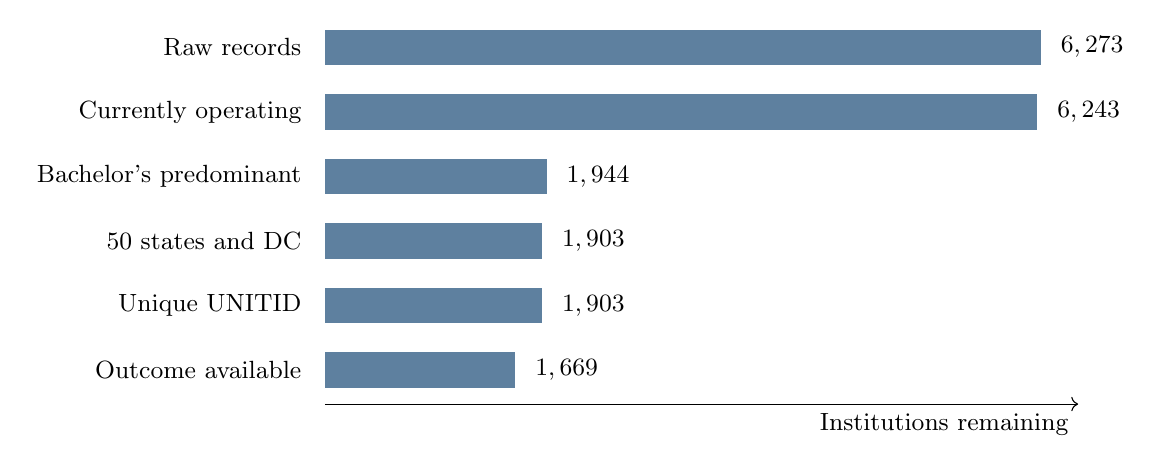
\begin{tikzpicture}[x=0.00145cm,y=0.82cm]
  \foreach \name/\value/\y in {
    {Raw records}/6273/5,
    {Currently operating}/6243/4,
    {Bachelor's predominant}/1944/3,
    {50 states and DC}/1903/2,
    {Unique UNITID}/1903/1,
    {Outcome available}/1669/0}
  {
    \fill[MainBlue!72] (0,\y) rectangle (\value,\y+0.55);
    \node[anchor=east,font=\small] at (-120,\y+0.275) {\name};
    \node[anchor=west,font=\small] at (\value+90,\y+0.275) {\pgfmathprintnumber[1000 sep={,}]{\value}};
  }
  \draw[->] (0,-0.25) -- (6600,-0.25) node[anchor=north east,font=\small] {Institutions remaining};
\end{tikzpicture}
\tabnote{Counts come from the latest fully executed notebook and the frozen Scorecard source.}
\end{figure}

\subsection{Variables and Data Dictionary}

The outcome, \sourcecode{C150_4_POOLED_SUPP}, is the pooled proportion completing within 150\% of normal program length. Calculations use the 0--1 scale; selected tables and prose convert values to percentages for interpretation. Table~\ref{tab:dictionary} defines the variables used in analysis.

\small
\begin{longtable}{>{\raggedright\arraybackslash}p{0.17\textwidth}>{\raggedright\arraybackslash}p{0.32\textwidth}>{\raggedright\arraybackslash}p{0.17\textwidth}>{\raggedright\arraybackslash}p{0.18\textwidth}}
\caption{Analysis Data Dictionary}\label{tab:dictionary}\\
\toprule
\textbf{Variable} & \textbf{Definition} & \textbf{Missing-Data Treatment} & \textbf{Analysis Role}\\
\midrule
\endfirsthead
\multicolumn{4}{l}{\textbf{Table \thetable\ continued}}\\
\toprule
\textbf{Variable} & \textbf{Definition} & \textbf{Missing-Data Treatment} & \textbf{Analysis Role}\\
\midrule
\endhead
\path{UNITID} & Federal institutional identifier & Uniqueness required & Audit key; excluded from fitting\\
\rowcolor{SoftGray}\path{INSTNM} & Reported institutional name & Retained as supplied & Output label; not a feature\\
\path{C150_4_POOLED_SUPP} & Pooled completion within 150\% of normal time, 0--1 & Observation required & Primary outcome\\
\rowcolor{SoftGray}\path{C150_4} & Unpooled completion within 150\% of normal time, 0--1 & No imputation & Sensitivity outcome\\
\path{NET_PRICE} & Public value from \path{NPT4_PUB}; otherwise \path{NPT4_PRIV} & Training-fold median plus indicator & Source cost measure\\
\rowcolor{SoftGray}\path{LOG_NET_PRICE} & $\log(1+\text{NET\_PRICE})$ & Derived after range checks & Affordability feature\\
\path{PCTPELL} & Undergraduate share receiving a Pell Grant & Training-fold median plus indicator & Need-related feature\\
\rowcolor{SoftGray}\path{PCTFLOAN} & Undergraduate share receiving a federal loan & Training-fold median; redundant flag removed & Financing feature\\
\path{LOG_UGDS} & $\log(1+\text{undergraduate enrollment})$ & Complete in analytical sample & Institutional size\\
\rowcolor{SoftGray}\path{ADM_RATE_SUPP} & Suppression-adjusted admission rate & Training-fold median plus indicator & Selectivity measure\\
\path{LOG_INEXPFTE} & Log of one plus instructional expenditure per FTE & Complete in analytical sample & Resource feature\\
\rowcolor{SoftGray}\path{LOG_AVGFACSAL} & Log of one plus average monthly faculty salary & Training-fold median plus indicator & Resource feature\\
\path{STUFACR} & Students per instructional faculty member & Complete in analytical sample & Staffing feature\\
\rowcolor{SoftGray}\path{CONTROL_LABEL} & Public, private nonprofit, private for-profit & Training-fold mode if absent & Feature and RQ2 factor\\
\path{REGION_LABEL} & IPEDS geographic region & Training-fold mode if absent & Geographic control\\
\rowcolor{SoftGray}\path{LOCALE4} & City, suburb, town, or rural & Training-fold mode if absent & Feature and RQ2 factor\\
\bottomrule
\end{longtable}
\normalsize

\subsection{Data Cleaning and Quality Checks}

Only the 19 source columns needed for screening or analysis were read from the 3,308-column file. Federal disclosure-suppression strings were converted to missing values, and numeric fields were parsed explicitly. Rates outside 0--1 and negative counts, dollar amounts, or ratios were flagged. None of the retained analytical values violated the specified ranges. Net price was selected from the public or private field according to institutional control, and detailed locale codes were collapsed into city, suburb, town, and rural categories.

Admission rate had the largest missing share: 223 colleges, or 13.36\%. Net price was absent for 34 institutions (2.04\%), faculty salary for 17 (1.02\%), and the Pell and loan shares for four each (0.24\%). The response, enrollment, instructional expenditure, student-faculty ratio, control, region, and locale were complete. The Pell and loan missingness indicators were identical, so the duplicate loan indicator was removed from the statistical design. Predictive preprocessing estimated medians, modes, scaling parameters, and category encodings inside each training fold. This prevented validation and test records from contributing to preprocessing.

Net price, enrollment, instructional expenditure, and faculty salary entered the models as $\log(1+x)$. Enrollment skewness changed from 6.693 to $-.196$, and faculty-salary skewness changed from 1.163 to $-.658$. Instructional expenditure remained irregular because several genuine records were extremely large or zero. These values were not deleted on appearance alone. HC3 inference, influence diagnostics, complete-case analysis, and training-derived percentile clipping were used to assess their effect.

\subsection{Exploratory Data Analysis}

The mean pooled completion rate was .5527 ($SD=.1909$), and the median was .5581. The middle half of colleges ranged from .4299 to .6835. Average net price was \$21,193, with a median of \$20,146. The median Pell share was .3279, the median federal-loan share was .4498, and the median admission rate was .7666. Typical institutional size was 1,839 undergraduates. Median instructional expenditure per full-time-equivalent student was \$10,551, median monthly faculty salary was \$8,485, and the median student-faculty ratio was 13.

Private nonprofit colleges formed 62.43\% of the sample ($n=1,042$), public colleges 33.13\% ($n=553$), and private for-profit colleges 4.43\% ($n=74$). Locale counts were 825 city, 391 suburb, 314 town, and 139 rural institutions. These imbalances affect the precision of group comparisons. Only 15 for-profit institutions entered the holdout, so the prespecified $n\geq20$ rule suppressed their predictive subgroup metrics.

Figure~\ref{fig:distribution} shows the broad completion distribution. The response spans nearly the full 0--1 scale, supporting continuous regression rather than an artificial high-low classification. A mean-only prediction cannot represent colleges near both ends of the distribution.

\begin{figure}[H]
\caption{Distribution of Pooled Six-Year Graduation Rates}\label{fig:distribution}
\centering
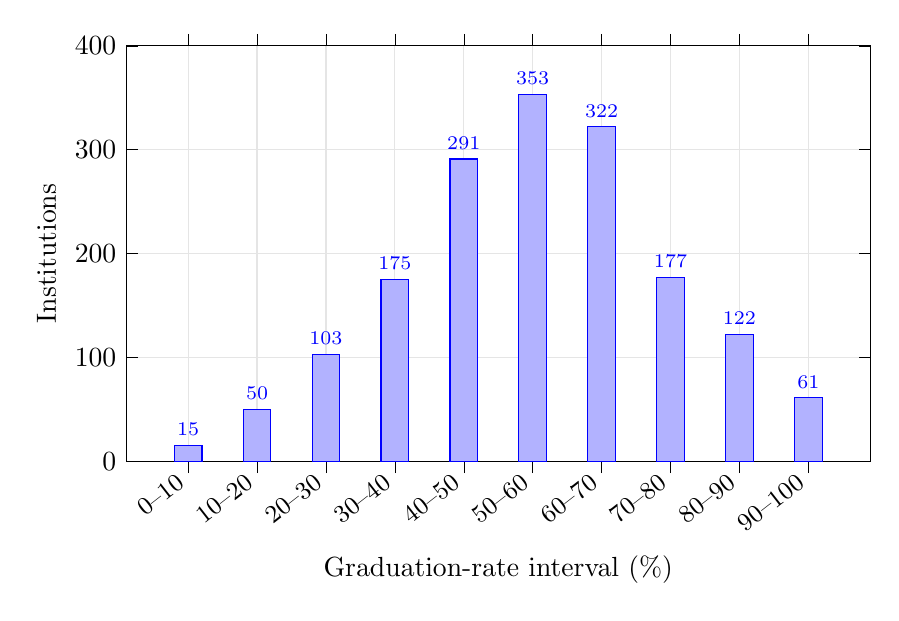
\begin{tikzpicture}
\begin{axis}[
  width=0.91\textwidth,height=2.7in,
  ybar,bar width=10pt,
  xlabel={Graduation-rate interval (\%)},ylabel={Institutions},
  symbolic x coords={0--10,10--20,20--30,30--40,40--50,50--60,60--70,70--80,80--90,90--100},
  xtick=data,x tick label style={rotate=38,anchor=east,font=\small},
  ymin=0,ymax=400,grid=major,grid style={gray!20},
  axis line style={black},tick style={black},
  nodes near coords,nodes near coords style={font=\scriptsize},
  every axis plot/.append style={fill=MainBlue!72,draw=MainBlue!85}]
\addplot coordinates {(0--10,15) (10--20,50) (20--30,103) (30--40,175) (40--50,291) (50--60,353) (60--70,322) (70--80,177) (80--90,122) (90--100,61)};
\end{axis}
\end{tikzpicture}
\tabnote{The ten bin counts sum to the complete analytical sample of 1,669 institutions.}
\end{figure}

The raw correlations in Figure~\ref{fig:correlations} show why single-predictor interpretations are inadequate. Completion correlated positively with faculty salary ($r=.589$), instructional expenditure ($r=.480$), and net price ($r=.400$). Pell share had a negative correlation of $r=-.594$, followed by admission rate ($r=-.460$), student-faculty ratio ($r=-.200$), and federal-loan share ($r=-.150$). These bivariate relationships combine several institutional differences that are addressed more directly in the adjusted and predictive models.

\begin{figure}[H]
\caption{Selected Raw Correlations With Pooled Graduation}\label{fig:correlations}
\centering
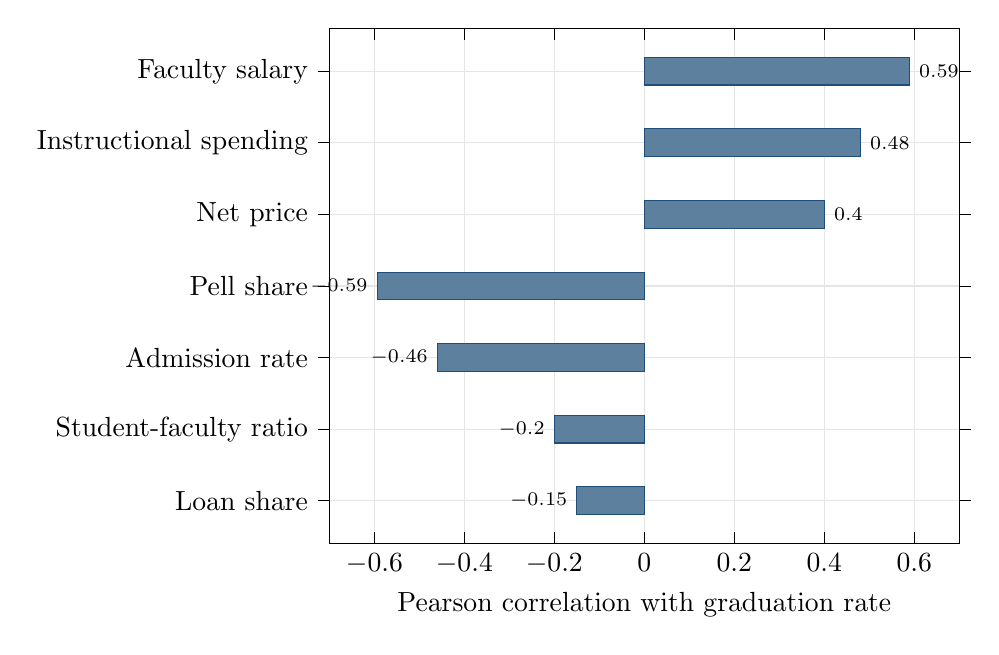
\begin{tikzpicture}
\begin{axis}[
  xbar,width=0.79\textwidth,height=3.2in,
  xmin=-0.70,xmax=0.70,
  xlabel={Pearson correlation with graduation rate},
  symbolic y coords={Loan share,Student-faculty ratio,Admission rate,Pell share,Net price,Instructional spending,Faculty salary},
  ytick=data,grid=major,grid style={gray!20},
  axis line style={black},tick style={black},
  visualization depends on={x \as \myx},
  nodes near coords={\pgfmathprintnumber[fixed,precision=2]{\myx}},
  nodes near coords align={horizontal},
  point meta=x,
  every node near coord/.append style={font=\scriptsize}]
\addplot[draw=MainBlue,fill=MainBlue!72] coordinates {(-0.150,Loan share) (-0.200,Student-faculty ratio) (-0.460,Admission rate) (-0.594,Pell share) (0.400,Net price) (0.480,Instructional spending) (0.589,Faculty salary)};
\end{axis}
\end{tikzpicture}
\tabnote{Correlations are descriptive and precede multivariable adjustment.}
\end{figure}

\subsection{Research Hypotheses and Minimum Sample Size}

All inferential tests used two-sided $\alpha=.05$. Prospective calculations targeted power of .80, with effect sizes fixed before the final holdout results were interpreted and calculations implemented in G*Power 3.1 (Faul et al., 2009). For RQ1 and RQ4, incremental regression effect size was defined as

\begin{equation}
f^2=\frac{R^2_{\text{full}}-R^2_{\text{reduced}}}{1-R^2_{\text{full}}}.
\end{equation}

With three tested affordability variables and as many as 20 full-model parameters, $f^2=.05$ required $N=223$ for RQ1. The more conservative $f^2=.03$ required $N=368$ for RQ4. For RQ2, Cohen's $f=.20$ required 277 observations for four locale groups and 244 for three control groups; 277 therefore governed. RQ3 used Fisher's transformation for an anticipated observed-predicted correlation of $r=.25$:

\begin{equation}
N=\left[\frac{z_{1-\alpha/2}+z_{1-\beta}}{\operatorname{atanh}(r)}\right]^2+3.
\end{equation}

Substituting 1.96, .842, and .25 gives 123.32, rounded upward to 124 independent test cases. Table~\ref{tab:power} confirms that every threshold was met.

\begin{table}[H]
\caption{Minimum Sample Sizes and Available Observations}\label{tab:power}
\centering
\begin{tabular}{lrrl}
\toprule
\textbf{Question} & \textbf{Minimum $N$} & \textbf{Available $N$} & \textbf{Decision}\\
\midrule
RQ1 & 223 & 1,669 & Requirement met\\
RQ2 & 277 & 1,669 & Requirement met\\
RQ3 & 124 test & 334 test & Requirement met\\
RQ4 & 368 & 1,669 & Requirement met\\
\bottomrule
\end{tabular}
\tabnote{The larger locale threshold governs RQ2; the untouched holdout governs RQ3.}
\end{table}

Appendix B maps each research question to its primary method, evidence, and decision rule.

\subsection{Statistical and Machine Learning Methods}

\subsubsection{RQ1 Robust Adjusted Regression}

Ordinary least squares was used because its coefficients and joint block test directly answer the adjusted-association question. The full model contained the three affordability variables, five numeric institutional controls, control, region, locale, and nonredundant missingness indicators. The reduced model omitted only affordability. A heteroskedasticity-consistent type 3 Wald/F test evaluated the three coefficients together. The partial \Rtwo\ compared the full and reduced fits. Variance inflation factors, the Breusch-Pagan test, residual plots, leverage, and Cook's distance described model behavior. A logit-transformed outcome and an influence-screen analysis checked whether the Pell direction depended on the primary form.

\subsubsection{RQ2 Adjusted Marginal Means}

The RQ2 analysis used the same analysis of covariance specification and HC3 covariance. Marginal means were obtained by setting each institution to a comparison category in turn while averaging over the observed covariate distribution. Separate global tests assessed control and locale. Pairwise contrasts came from the fitted covariance matrix, with Holm adjustment for multiplicity and simultaneous confidence intervals for the size and direction of each comparison.

\subsubsection{RQ3 Model Comparison}

The analytical sample was split once with seed 640 into 1,335 training and 334 test institutions. Stratification used institutional control and graduation-rate quintile when cell sizes permitted. Five fixed folds inside the training data were reused for every candidate. Numeric imputation, missingness indicators, robust scaling for elastic net, and one-hot encoding were learned separately inside each training fold.

The candidates were ordinary least squares, elastic net, random forest, and gradient boosting. Each tuned model family received a 12-configuration full grid. Mean training-fold root mean squared error determined the selected class. The test set was evaluated only after that decision. A reference model assigned the training mean to every holdout institution. The main metrics were

\begin{align}
\operatorname{MAE} &= \frac{1}{n}\sum_{i=1}^{n}|y_i-\hat y_i|,\\
\operatorname{RMSE} &= \sqrt{\frac{1}{n}\sum_{i=1}^{n}(y_i-\hat y_i)^2},\\
R^2 &= 1-\frac{\sum_{i=1}^{n}(y_i-\hat y_i)^2}{\sum_{i=1}^{n}(y_i-\bar y)^2}.
\end{align}

The prespecified usefulness standard required positive test \Rtwo, at least a 10\% reduction in RMSE relative to the training-mean reference, reasonably stable cross-validation error, and no reported subgroup RMSE above 1.5 times the overall selected-model RMSE.

\subsubsection{RQ4 Incremental Predictive Value}

RQ4 retained the model class selected from training cross-validation. The full version used all eleven features. The reduced version removed log net price, Pell share, and federal-loan share while retaining the same model class, folds, tuning effort, and evaluation institutions. Incremental performance was expressed as

\begin{equation}
\Delta R^2=R^2_{\text{full}}-R^2_{\text{reduced}}
\end{equation}

and as the percentage RMSE reduction achieved by the full specification. Each fold yielded a matched pair of full and reduced errors. Paired $t$ tests and Wilcoxon signed-rank tests were reported, with the low resolution of a five-pair nonparametric test stated explicitly.

\subsubsection{Uncertainty Explanation and Sensitivity Analysis}

Cross-validation-plus (CV+) conformal prediction intervals were constructed from the five training folds and checked against 95\% coverage on the holdout. Average width was reported because high coverage can be obtained through intervals that are too broad to guide a single case. Permutation importance measured the increase in test RMSE after one feature was shuffled. Partial-dependence plots described average fitted patterns for the leading numeric variables.

Subgroup performance was reported only when at least 20 test institutions were available. The audit included MAE, RMSE, \Rtwo, mean residual, and interval coverage for control and locale groups. Three planned sensitivity runs used complete predictor cases, training-derived first/99th percentile clipping, and the unpooled \sourcecode{C150_4} outcome.

\section{Architecture Diagram and Workflow}

\subsection{System Overview}

One executed notebook takes the named College Scorecard release through source verification, eligibility screening, feature construction, exploratory analysis, statistical inference, predictive model selection, holdout evaluation, uncertainty analysis, and export. The workflow keeps the inferential and predictive questions distinct while preserving one documented dataset and set of definitions.

\subsection{Architecture Diagram}

Figure~\ref{fig:workflow} shows the full sequence and marks the point at which holdout evaluation begins. All model selection and preprocessing decisions occur within training data before the test institutions are used.

\begin{figure}[H]
\caption{End-to-End Workflow of the Proposed System}\label{fig:workflow}
\centering
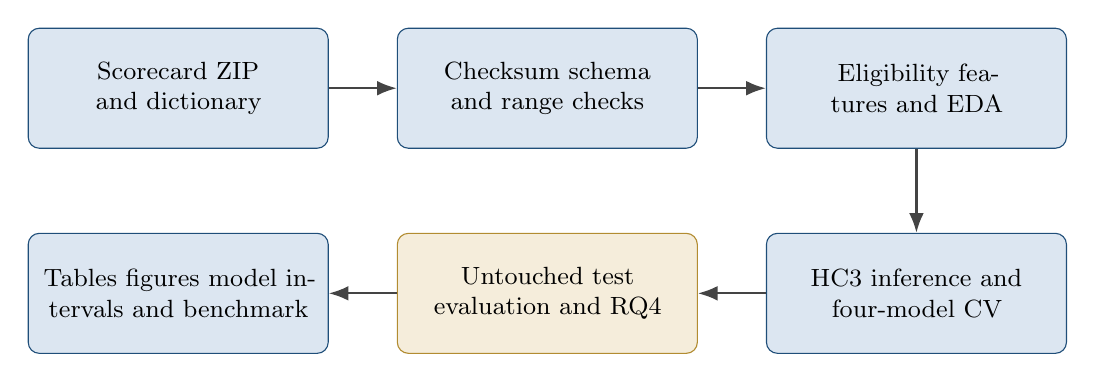
\begin{tikzpicture}[
  node distance=0.42in and 0.34in,
  box/.style={rectangle,rounded corners,draw=MainBlue,fill=LightBlue,minimum width=1.50in,minimum height=0.60in,text width=1.35in,align=center,font=\small},
  hold/.style={rectangle,rounded corners,draw=WarmGold!90!black,fill=WarmGold!18,minimum width=1.50in,minimum height=0.60in,text width=1.35in,align=center,font=\small},
  arrow/.style={-{Latex[length=2.5mm]},thick,draw=DarkGray}]
\node[box] (source) {Scorecard ZIP and dictionary};
\node[box,right=of source] (verify) {Checksum schema and range checks};
\node[box,right=of verify] (prepare) {Eligibility features and EDA};
\node[box,below=of prepare] (train) {HC3 inference and four-model CV};
\node[hold,left=of train] (test) {Untouched test evaluation and RQ4};
\node[box,left=of test] (export) {Tables figures model intervals and benchmark};
\draw[arrow] (source) -- (verify);
\draw[arrow] (verify) -- (prepare);
\draw[arrow] (prepare) -- (train);
\draw[arrow] (train) -- (test);
\draw[arrow] (test) -- (export);
\end{tikzpicture}
\tabnote{Blue boxes cover data preparation and model development. The gold box marks the first use of the frozen holdout.}
\end{figure}

\subsection{Workflow Components}

\subsubsection{Data Ingestion}

The ingestion stage stores the official source location, retrieval time, release-specific filename, file sizes, and SHA-256 digests. It verifies the required field names before loading only the columns needed for eligibility and analysis. The data dictionary's cohort-map worksheet records the reporting period attached to each field.

\subsubsection{Data Preprocessing}

Preprocessing applies the eligibility filters in their recorded order, converts suppressed entries to missing values, validates allowable ranges, constructs net price and transformed variables, and assigns readable control, region, and locale labels. The 1,669-row analytical file is then written in identifier order. Predictive imputation and encoding remain inside the validation pipeline.

\subsubsection{Exploratory Data Analysis}

Exploration reports continuous distributions, categorical counts, missingness, transformations, and raw correlations. Each display serves a later analytical decision: the response distribution supports regression, skewness supports the four log transformations, group counts govern subgroup reporting, and predictor correlations support multivariable modeling.

\subsubsection{Feature Engineering}

The full model contains log net price, Pell share, federal-loan share, log enrollment, admission rate, log instructional expenditure, log faculty salary, student-faculty ratio, control, region, and locale. The reduced RQ4 model removes only the first three features. No completion-derived variable, retention field, student identifier, or demographic subgroup outcome is used as a predictor.

\subsubsection{Model Development}

The training branch fixes the 80/20 split, creates five common folds, applies fold-specific preprocessing, searches the three tuned grids, and compares mean validation errors. Ordinary least squares provides an untuned reference. The selected model is then fitted to the entire training set.

\subsubsection{Model Evaluation}

Evaluation applies each completed pipeline to the 334 institutions excluded from training. The notebook saves institution-level predictions, residuals, model metrics, success-rule checks, the full-versus-reduced comparison, conformal intervals, and subgroup results. The selected estimator and its preprocessing steps are serialized together so later use cannot silently change the feature order or imputation rule.

\subsubsection{Deployment}

The project produces a read-only benchmark file rather than a public ranking service. Each holdout row contains observed completion, expected completion, their difference, a 95\% interval, the peer definition and size, peer mean and median, source date, model version, and an intended-use statement. A later dashboard can display this file after a new release passes schema, range, inclusion-flow, and validation checks.

\subsection{Tools and Technologies}

The notebook was executed with Python 3.12.14 on a Linux central processing unit environment. pandas and NumPy handled data preparation; SciPy and statsmodels supplied inference; scikit-learn supplied preprocessing, validation, and predictive models; Matplotlib and Seaborn produced figures; Joblib serialized the fitted pipeline. The report was authored in \LaTeX. No graphics processing unit, paid dataset, participant recruitment, or proprietary modeling service was required.

\section{Results}

\subsection{Model Performance}

Random forest had the lowest mean training-fold RMSE at .10716. Gradient boosting was close at .10822; elastic net and ordinary least squares produced .11913 and .11920. Because selection used validation results, the small random-forest advantage was recorded before any holdout comparison. Figure~\ref{fig:cv} displays both the mean and one standard deviation across the five folds.

\begin{figure}[H]
\caption{Five-Fold Cross-Validated Model Comparison}\label{fig:cv}
\centering
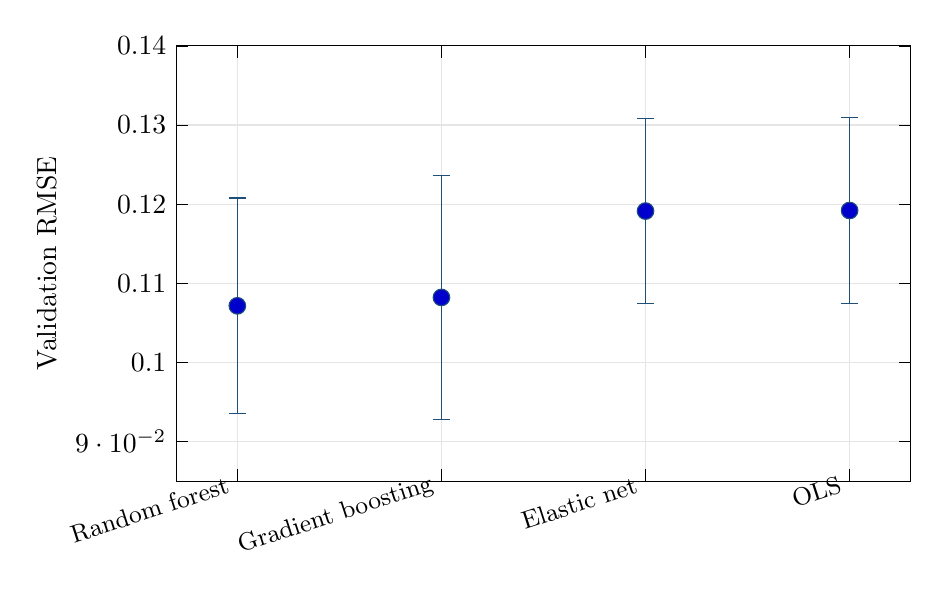
\begin{tikzpicture}
\begin{axis}[
  width=0.90\textwidth,height=2.8in,
  ylabel={Validation RMSE},
  symbolic x coords={Random forest,Gradient boosting,Elastic net,OLS},
  xtick=data,x tick label style={rotate=18,anchor=east,font=\small},
  ymin=0.085,ymax=0.14,grid=major,grid style={gray!20},
  axis line style={black},tick style={black},
  error bars/y dir=both,error bars/y explicit]
\addplot+[only marks,mark=*,mark size=3pt,color=MainBlue,error bars/.cd,y dir=both,y explicit] coordinates {
  (Random forest,0.10716) +- (0,0.01362)
  (Gradient boosting,0.10822) +- (0,0.01537)
  (Elastic net,0.11913) +- (0,0.01169)
  (OLS,0.11920) +- (0,0.01178)};
\end{axis}
\end{tikzpicture}
\tabnote{Points are mean validation RMSE; error bars are $\pm1$ standard deviation across the five fixed training folds.}
\end{figure}

All four fitted models were evaluated on the same 334 holdout colleges. Table~\ref{tab:testmetrics} reports the common metrics. Random forest produced MAE of .06720, RMSE of .09131, \Rtwo\ of .76769, and observed-predicted $r=.87701$. Relative to the training-mean RMSE of .18946, it reduced RMSE by 51.81\%. Gradient boosting was the closest alternative, with RMSE .09362 and \Rtwo\ .75577. The two linear models explained about 70\% of holdout variation.

\begin{table}[H]
\caption{Model Performance on the Frozen 334-Institution Test Set}\label{tab:testmetrics}
\centering
\begin{tabular}{lrrrrl}
\toprule
\textbf{Model} & \textbf{MAE} & \textbf{RMSE} & \textbf{\Rtwo} & \textbf{$r$} & \textbf{Role}\\
\midrule
Mean baseline & .15213 & .18946 & $-.00024$ & -- & Training-mean reference\\
OLS & .07770 & .10372 & .70022 & .83725 & Linear comparator\\
Elastic net & .07752 & .10331 & .70259 & .83876 & Regularized comparator\\
\rowcolor{LightBlue}Random forest & \textbf{.06720} & \textbf{.09131} & \textbf{.76769} & \textbf{.87701} & Selected by CV\\
Gradient boosting & .06983 & .09362 & .75577 & .86959 & Nonlinear comparator\\
\bottomrule
\end{tabular}
\tabnote{The four fitted-model correlation $p$ values were below .001. Selection was based on training-fold RMSE rather than holdout performance.}
\end{table}

\subsection{Visual Evidence}

Figure~\ref{fig:testbars} places the holdout errors on a percentage-point scale. The two ensemble models have the lowest MAE and RMSE, while the mean reference is substantially worse. The comparison also shows that MAE and RMSE are not interchangeable: RMSE is larger because it gives more weight to the less frequent large misses.

\begin{figure}[H]
\caption{Holdout Mean Absolute Error and Root Mean Squared Error}\label{fig:testbars}
\centering
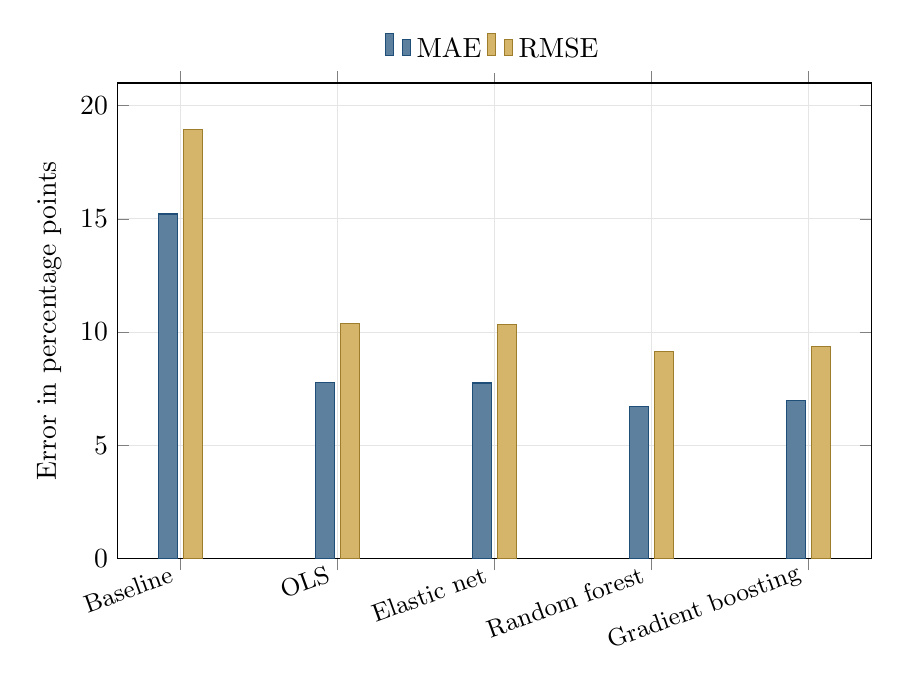
\begin{tikzpicture}
\begin{axis}[
  ybar,width=0.92\textwidth,height=3.0in,
  bar width=7pt,
  ylabel={Error in percentage points},
  symbolic x coords={Baseline,OLS,Elastic net,Random forest,Gradient boosting},
  xtick=data,x tick label style={rotate=20,anchor=east,font=\small},
  ymin=0,ymax=21,grid=major,grid style={gray!20},
  legend style={at={(0.5,1.02)},anchor=south,legend columns=2,draw=none}]
\addplot[fill=MainBlue!72,draw=MainBlue] coordinates {(Baseline,15.213) (OLS,7.770) (Elastic net,7.752) (Random forest,6.720) (Gradient boosting,6.983)};
\addplot[fill=WarmGold!75,draw=WarmGold!80!black] coordinates {(Baseline,18.946) (OLS,10.372) (Elastic net,10.331) (Random forest,9.131) (Gradient boosting,9.362)};
\legend{MAE,RMSE}
\end{axis}
\end{tikzpicture}
\tabnote{Errors were calculated on one common, untouched holdout.}
\end{figure}

\subsection{Results by Research Question}

\subsubsection{RQ1 Affordability}

The HC3 joint test rejected the null that the three affordability coefficients were all zero, $F(3,1643)=59.80418$, $p=1.081\times10^{-36}$. The full regression had \Rtwo\ .64700 and adjusted \Rtwo\ .64163. Without affordability, \Rtwo\ fell to .57976. The resulting \DeltaRtwo\ was .06724, and partial \Rtwo\ was .16001. Affordability therefore carried adjusted information beyond the measured institutional covariates.

The individual estimates were more qualified. Pell share had coefficient $b=-.34634$, HC3 $SE=.04074$, $t=-8.50148$, $p<.001$, 95\% CI [$-.42625,-.26643$], and standardized $\beta=-.29672$. A .10 difference in Pell share corresponded to a 3.46 percentage-point difference in expected institutional completion when the other model terms were held constant. This is a comparison between colleges serving different concentrations of financial need. It does not estimate what happens to an individual after receiving a Pell Grant.

Log net price was positive but uncertain, $b=.02268$, $SE=.01269$, $p=.07416$, 95\% CI [$-.00222,.04758$]. Federal-loan share was also unresolved, $b=-.02050$, $SE=.03019$, $p=.49724$, 95\% CI [$-.07971,.03871$]. Table~\ref{tab:rq1} reports the three coefficients.

\begin{table}[H]
\caption{HC3 Estimates for the Affordability Variables}\label{tab:rq1}
\centering
\small
\begin{tabular}{lrrrrrr}
\toprule
\textbf{Variable} & \textbf{$b$} & \textbf{HC3 SE} & \textbf{$t$} & \textbf{$p$} & \textbf{95\% CI} & \textbf{$\beta$}\\
\midrule
Log net price & .02268 & .01269 & 1.78675 & .07416 & [$-.00222,.04758$] & .05596\\
\rowcolor{LightBlue}Pell share & $-.34634$ & .04074 & $-8.50148$ & $<.001$ & [$-.42625,-.26643$] & $-.29672$\\
Federal-loan share & $-.02050$ & .03019 & $-.67899$ & .49724 & [$-.07971,.03871$] & $-.02217$\\
\bottomrule
\end{tabular}
\tabnote{The outcome is on the 0--1 scale. Standardized coefficients are reported for the affordability variables.}
\end{table}

The Breusch-Pagan test rejected constant variance, $LM=392.72265$, $F=20.22267$, both $p<.001$, supporting HC3 inference. The current executed notebook identifies 118 cases above the common $4/n$ Cook's-distance threshold; maximum Cook's distance is .39268 and maximum leverage is 1.00. High variance inflation factors for several region indicators reflect sparse categorical coding, including five cases in region code 0. The larger substantive numeric values were 3.068 for log faculty salary, 3.022 for log enrollment, 2.430 for log net price, and 2.305 for Pell share. The bounded-outcome and influence-screen checks preserved the negative Pell direction.

\subsubsection{RQ2 Control and Locale}

Adjusted completion differed by institutional control, $F(2,1643)=37.79805$, $p=8.932\times10^{-17}$, partial $\eta^2=.04399$. Estimated marginal means were 58.37\% for private nonprofits, 49.39\% for public colleges, and 55.63\% for private for-profits. Private nonprofits exceeded public colleges by 8.98 points, simultaneous 95\% CI [6.50, 11.45], Holm $p<.001$. The for-profit estimate exceeded the public estimate by 6.24 points, CI [.40, 12.08], Holm $p=.02108$. The 2.74-point difference between private for-profits and private nonprofits was not resolved, Holm $p=.23462$.

Locale did not reach the .05 criterion after the same adjustment, $F(3,1643)=1.45581$, $p=.22484$, partial $\eta^2=.00265$. Means were 55.64\% for city, 55.57\% for suburb, 54.82\% for town, and 53.27\% for rural colleges. Every Holm-adjusted locale interval included zero. The largest point difference, city minus rural at 2.37 points, remained uncertain. Figure~\ref{fig:means} shows the estimates and HC3 confidence intervals.

\begin{figure}[H]
\caption{Adjusted Graduation Means With 95 Percent HC3 Confidence Intervals}\label{fig:means}
\centering
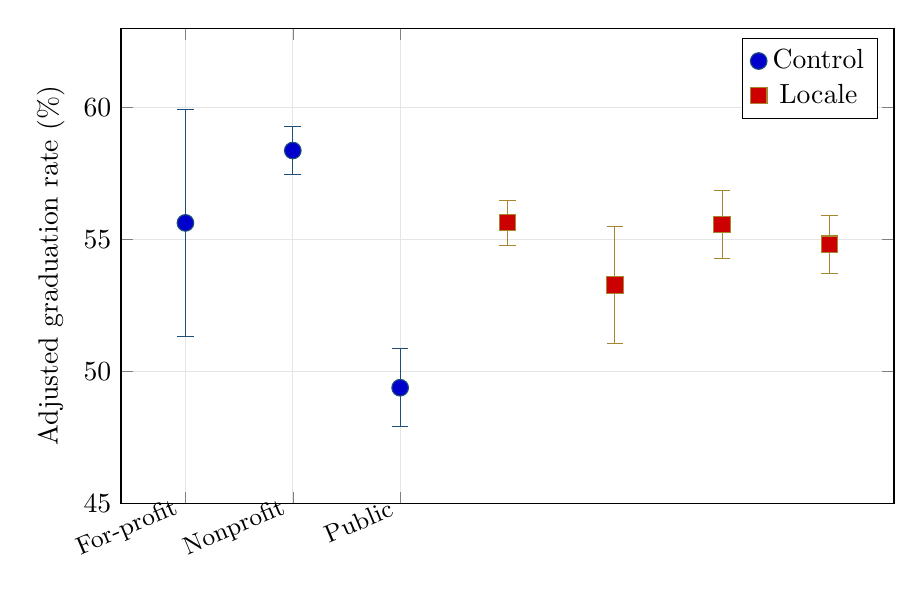
\begin{tikzpicture}
\begin{axis}[
  width=0.94\textwidth,height=3.0in,
  ymin=45,ymax=63,ylabel={Adjusted graduation rate (\%)},
  symbolic x coords={For-profit,Nonprofit,Public,City,Rural,Suburb,Town},
  xtick=data,x tick label style={rotate=23,anchor=east,font=\small},
  grid=major,grid style={gray!20},
  error bars/y dir=both,error bars/y explicit]
\addplot+[only marks,mark=*,mark size=3pt,color=MainBlue,error bars/.cd,y dir=both,y explicit] coordinates {
  (For-profit,55.63) +- (0,4.29)
  (Nonprofit,58.37) +- (0,0.92)
  (Public,49.39) +- (0,1.48)};
\addplot+[only marks,mark=square*,mark size=3pt,color=WarmGold!85!black,error bars/.cd,y dir=both,y explicit] coordinates {
  (City,55.64) +- (0,0.85)
  (Rural,53.27) +- (0,2.22)
  (Suburb,55.57) +- (0,1.30)
  (Town,54.82) +- (0,1.10)};
\legend{Control,Locale}
\end{axis}
\end{tikzpicture}
\tabnote{Intervals are based on the robust fitted covariance matrix. The for-profit estimate is less precise because the analytical group contains 74 institutions.}
\end{figure}

\subsubsection{RQ3 Prediction}

RQ3 met the practical alternative. Random forest produced positive test \Rtwo\ of .76769, observed-predicted $r=.87701$, and RMSE 51.81\% below the training-mean reference. All four fitted models beat that reference. The selected model also satisfied the stability rule: its cross-validation RMSE coefficient of variation was .127. The highest reported subgroup RMSE was below the prespecified 1.5-times-overall limit.

The two error measures describe different features of performance. MAE .06720 means that the average absolute miss was about 6.72 percentage points. RMSE .09131 is larger because it weights the relatively large misses more heavily. The model is useful for contextual review, but an individual college prediction requires its interval and local evidence.

\subsubsection{RQ4 Added Predictive Value of Affordability}

The full random forest achieved MAE .06720, RMSE .09131, and \Rtwo\ .76769. The reduced model without net price, Pell share, and loan share produced MAE .08099, RMSE .11192, and \Rtwo\ .65093. Adding affordability lowered RMSE by 18.42\% relative to the reduced model and produced \DeltaRtwo\ .11675.

All five matched validation folds favored the full set. Mean reduced-minus-full RMSE was .00992, 95\% CI [.00343, .01641], paired $t$ $p=.01322$. The corresponding MAE difference was .00770, CI [.00307, .01234], $p=.00992$. Both Wilcoxon tests produced $p=.0625$. With only five pairs, that test has coarse probability steps, so the consistent fold direction and effect estimates are more informative than a binary interpretation of the Wilcoxon result.

Permutation importance agreed with the block comparison. Shuffling Pell share increased test RMSE by .05743, the largest change for any single feature. Instructional expenditure followed at .02873, then admission rate (.01957), faculty salary (.01307), log net price (.00879), enrollment (.00867), loan share (.00262), control (.00204), region (.00182), student-faculty ratio (.00158), and locale (.00088). Figure~\ref{fig:importance} reports the ordering.

\begin{figure}[H]
\caption{Permutation Importance on Unseen Institutions}\label{fig:importance}
\centering
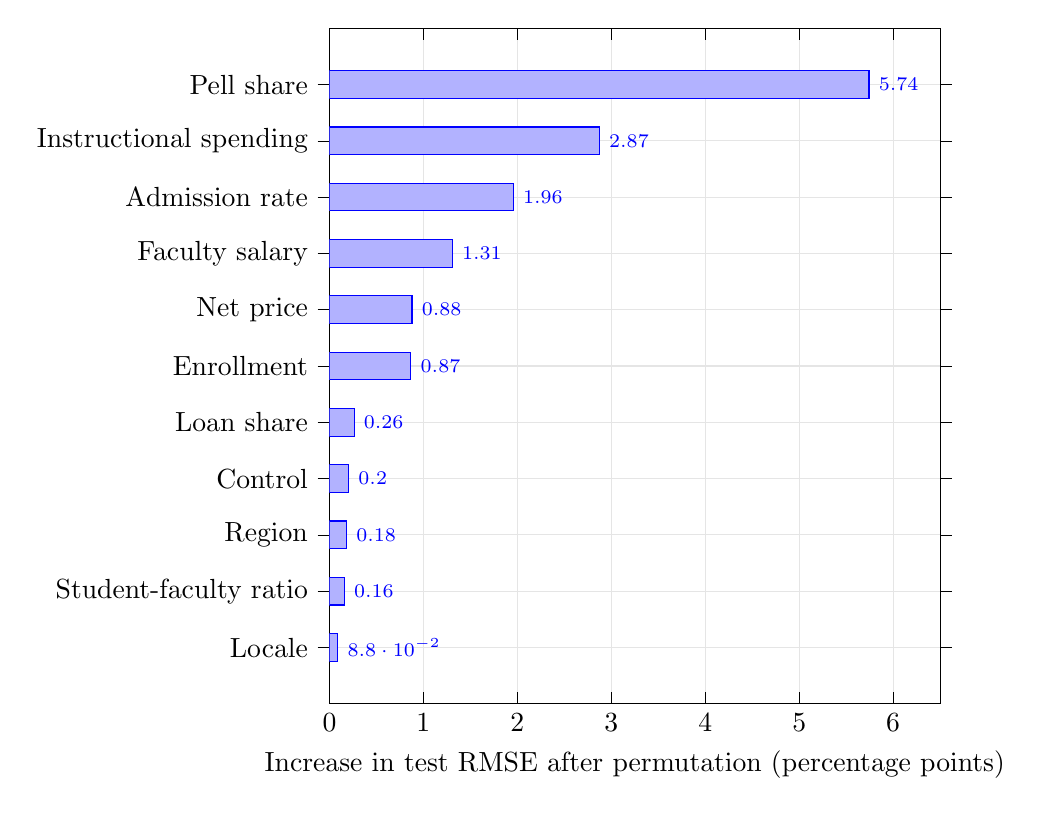
\begin{tikzpicture}
\begin{axis}[
  xbar,width=0.77\textwidth,height=4.0in,
  xmin=0,xmax=6.5,
  xlabel={Increase in test RMSE after permutation (percentage points)},
  symbolic y coords={Locale,Student-faculty ratio,Region,Control,Loan share,Enrollment,Net price,Faculty salary,Admission rate,Instructional spending,Pell share},
  ytick=data,grid=major,grid style={gray!20},
  axis line style={black},tick style={black},
  nodes near coords,nodes near coords style={font=\scriptsize},
  every axis plot/.append style={fill=MainBlue!72,draw=MainBlue}]
\addplot coordinates {(0.088,Locale) (0.158,Student-faculty ratio) (0.182,Region) (0.204,Control) (0.262,Loan share) (0.867,Enrollment) (0.879,Net price) (1.307,Faculty salary) (1.957,Admission rate) (2.873,Instructional spending) (5.743,Pell share)};
\end{axis}
\end{tikzpicture}
\tabnote{Importance is predictive dependence, not causal importance. Correlated features may divide credit when one feature is shuffled.}
\end{figure}

\subsection{Uncertainty Subgroups and Sensitivity Results}

The CV+ intervals achieved 97.904\% empirical coverage against a nominal 95\% target. Mean width was .44042, about 44.04 percentage points. The intervals were conservative but broad. Their width prevents a point prediction from being interpreted as a precise institutional target.

Table~\ref{tab:subgroups} reports groups meeting $n\geq20$. Public-college RMSE was .07948 and private-nonprofit RMSE was .09260. By locale, RMSE ranged from .07570 for towns to .11938 for rural institutions. Rural error was 1.31 times the overall RMSE and remained under the 1.50 threshold, although the rural result came from only 35 test institutions. Metrics for the 15 for-profit holdout colleges were suppressed.

\begin{table}[H]
\caption{Reported Subgroup Performance for Random Forest}\label{tab:subgroups}
\centering
\begin{tabular}{llrrrrr}
\toprule
\textbf{Factor} & \textbf{Group} & \textbf{$n$} & \textbf{MAE} & \textbf{RMSE} & \textbf{\Rtwo} & \textbf{Coverage}\\
\midrule
Control & Private nonprofit & 209 & .06639 & .09260 & .75209 & .97608\\
Control & Public & 110 & .06239 & .07948 & .79059 & 1.00000\\
\rowcolor{SoftGray}Locale & City & 158 & .07037 & .09008 & .78308 & .98101\\
Locale & Rural & 35 & .08292 & .11938 & .54712 & .94286\\
\rowcolor{SoftGray}Locale & Suburb & 79 & .06187 & .09059 & .79559 & .97468\\
Locale & Town & 62 & .05701 & .07570 & .75297 & 1.00000\\
\bottomrule
\end{tabular}
\tabnote{Private for-profit performance was withheld because the holdout subgroup contained 15 institutions.}
\end{table}

The complete-predictor-case model used 1,138 training and 287 test colleges and achieved MAE .06241, RMSE .08685, and \Rtwo\ .73758. Training-derived first/99th percentile clipping retained the 1,335/334 split and achieved MAE .06688, RMSE .09124, and \Rtwo\ .76803. The alternative \sourcecode{C150_4} outcome used 1,332 training and 334 test institutions and produced MAE .07131, RMSE .09433, and \Rtwo\ .75573. The exact metrics changed, but all three planned checks retained substantial unseen-college prediction.

\subsection{Overall Interpretation}

The four questions produce a coherent but bounded result. Affordability adds information in both the adjusted regression and the predictive feature-block comparison. Pell share carries most of the individual affordability signal, while log net price and federal-loan share are not individually resolved in the linear model. Control groups differ after adjustment, but the data do not distinguish locale means at the .05 level. Random forest reduces holdout error and meets the complete usefulness standard.

The selected model accounts for approximately 77\% of variation relative to the holdout mean, yet its RMSE is about nine percentage points and its average interval is much wider. Academic preparation, program mix, transfer behavior, work obligations, course access, local labor markets, and campus practice are among the omitted conditions that may contribute to the remaining error. The prediction is best used to narrow an institutional question rather than label a college.

\subsection{Practical Significance}

The benchmark lets an institutional research office compare an observed completion rate with two reference points: the model expectation and the mean for a plainly defined peer set. For example, Abraham Baldwin Agricultural College had observed completion of 32.51\%, model-expected completion of 43.32\%, and a peer mean of 47.12\%. The observed-minus-expected gap was $-10.81$ points, and the 95\% interval extended from 20.86\% to 65.99\%. The peer group contained 59 public, town-based colleges in the same enrollment quartile.

The wide interval does not support a performance label. It supports verification of the source row and a focused local review. A high-Pell institution might examine emergency aid, unpaid-balance holds, working hours, course scheduling, advising access, or return after stop-out. Only campus records can distinguish among these explanations.

\section{Implementation and User Benefit}

\subsection{Deployment Approach}

The proposed application is a read-only benchmark for institutional research and planning staff. The notebook already creates the input table. Each row includes the institution name and identifier, observed and expected completion, their difference, the CV+ interval, peer rule and count, peer mean and median, model version, data-release date, retraining trigger, prediction status, and intended-use notice.

Streamlit, Dash, Power BI, or Tableau could display the prepared file without changing the trained pipeline. The first implementation should remain internal. A new Scorecard release may alter field names, definitions, or reporting periods, so any refresh must begin with schema checks, range validation, an inspected inclusion flow, retraining, and comparison with the prior model. The current export identifies version QM640-v1.0 and the June 10, 2026 release. Review is scheduled for June 10, 2027 or immediately after a material source or schema change.

\subsection{System Integration}

The benchmark fits naturally within an existing institutional review. Staff select a college, examine its observed value and model expectation, and then decide whether approved campus data should be consulted. Local follow-up might use retention, earned credits, course completion, account balances, advising contacts, or stop-out timing. These student-level records must remain inside the institution's authorized environment and are not required by the national benchmark.

The serialized pipeline stores the estimator, preprocessing operations, feature order, and fitted parameters together. A dashboard reads saved predictions instead of recalculating them in browser code. This design reduces the risk that an interface will change an encoding or imputation rule while presenting the output as the original model.

\subsection{User Interaction}

The opening screen uses an institution selector and a concise comparison of observed completion, model expectation, and peer mean. It also presents the observed-minus-expected difference, 95\% interval, peer definition and size, release date, and model version. Figure~\ref{fig:dashboard} shows the numerical pattern for the demonstration institution.

\begin{figure}[H]
\caption{Notebook-Derived Contextual Benchmark With Prediction Interval}\label{fig:dashboard}
\centering
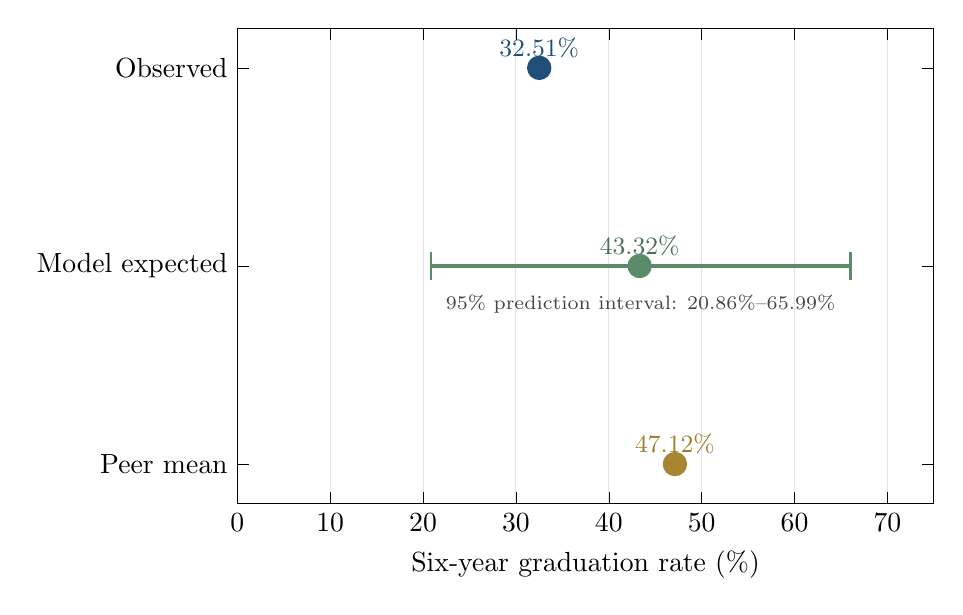
\begin{tikzpicture}
\begin{axis}[
  width=0.86\textwidth,height=3.0in,
  xmin=0,xmax=75,
  xlabel={Six-year graduation rate (\%)},
  symbolic y coords={Peer mean,Model expected,Observed},
  ytick={Peer mean,Model expected,Observed},
  xtick={0,10,20,30,40,50,60,70},
  xmajorgrids=true,ymajorgrids=false,grid style={gray!22},
  axis line style={black},tick style={black},clip=false]
\draw[MutedGreen,line width=1.4pt]
  (axis cs:20.86,Model expected) -- (axis cs:65.99,Model expected);
\draw[MutedGreen,line width=1.0pt]
  ([yshift=-5pt]axis cs:20.86,Model expected) -- ([yshift=5pt]axis cs:20.86,Model expected);
\draw[MutedGreen,line width=1.0pt]
  ([yshift=-5pt]axis cs:65.99,Model expected) -- ([yshift=5pt]axis cs:65.99,Model expected);
\addplot[only marks,mark=*,mark size=4.2pt,color=MainBlue] coordinates {(32.51,Observed)};
\addplot[only marks,mark=*,mark size=4.2pt,color=MutedGreen] coordinates {(43.32,Model expected)};
\addplot[only marks,mark=*,mark size=4.2pt,color=WarmGold!85!black] coordinates {(47.12,Peer mean)};
\node[anchor=south,font=\small,text=MainBlue] at (axis cs:32.51,Observed) {32.51\%};
\node[anchor=south,font=\small,text=MutedGreen!80!black] at (axis cs:43.32,Model expected) {43.32\%};
\node[anchor=south,font=\small,text=WarmGold!80!black] at (axis cs:47.12,Peer mean) {47.12\%};
\node[anchor=north,font=\scriptsize,text=DarkGray,yshift=-7pt]
  at (axis cs:43.425,Model expected) {95\% prediction interval: 20.86\%--65.99\%};
\end{axis}
\end{tikzpicture}

\small Abraham Baldwin Agricultural College; peer $n=59$.
\tabnote{Peers match control, locale, and undergraduate-enrollment quartile. The model provides association and comparison, not causation.}
\end{figure}

Peers first match control, locale, and enrollment quartile. If fewer than 20 peers remain, the system relaxes locale and records the broader rule. If that still leaves fewer than 20, control alone defines the comparison. The rule cannot be changed silently to produce a more favorable or unfavorable result.

\subsection{Benefits to Users}

The export saves analysts from rebuilding the Scorecard workflow for every institutional review. It applies one eligibility definition, transformation policy, split, and prediction procedure across the national sample. More importantly, it displays the point expectation beside its interval and peer summary, so the user can see that the estimate is not exact.

The model does not calculate return on investment or recommend spending. Any operational or financial benefit would come from a later campus investigation and a specific response supported by local evidence. For example, if a local analysis links stop-out to registration holds, the institution can estimate the cost and likely reach of a targeted policy with its own records. The national benchmark ends before that decision.

\subsection{Example Use Case}

Consider a public college in a town with 45\% pooled completion. Its model expectation is 53\%, its 95\% interval is 31\%--73\%, and its matched peers average 55\%. The observed rate is eight points below the model expectation, but the interval is too broad to classify the college as unusual.

An analyst would first verify the Scorecard row and the applicable completion cohort. The next review could examine first-year credit accumulation, gateway-course completion, unpaid balances, advising contacts, transfer-out, and the semester in which students stop attending. If departures cluster after the second year, a first-semester intervention would address the wrong stage. The benchmark has served its intended purpose once it defines this more precise local question.

\section{Limitations and Further Improvements}

\subsection{Limitations}

The design is cross-sectional and institution-level. Coefficients compare colleges conditional on recorded characteristics; they do not estimate the result of changing price, Pell share, spending, or another input at one campus. Pell share needs particular care because it describes institutional composition, while grant receipt belongs to a student. Moving between those levels would create an unsupported ecological conclusion.

College Scorecard fields come from several reporting periods and administrative sources. The cohort map documents their timing but cannot remove misalignment or reporting error. A merger, program change, correction, or organizational restructuring may also make a frozen record less representative. A checksum verifies the analyzed bytes, not the substantive accuracy of every value supplied to the agency.

Several plausible conditions are missing. The file does not fully represent prior academic preparation, program mix, transfer behavior, work hours, childcare, housing insecurity, course availability, advising quality, campus climate, or local economic conditions. A nonlinear estimator can model complicated relationships among observed features, but it cannot reconstruct a variable that was never recorded.

Subgroup evidence is uneven. The private for-profit group contains 74 analytical institutions and only 15 holdout cases, so its predictive metrics are not reported. Rural institutions pass the reporting threshold with 35 cases, yet their RMSE of .11938 exceeds the overall .09131. Aggregate accuracy does not establish equal reliability across every control or locale subgroup.

The conformal intervals limit one-college precision. Their coverage is 97.90\%, but their average width is about 44 percentage points. Suppressing the interval would make the point estimate look more precise than the evidence permits. Retaining it makes clear that some individual comparisons can guide inquiry but not classification.

Permutation importance and partial dependence describe the fitted model rather than an intervention. Correlated predictors may exchange importance when shuffled, and partial-dependence curves can average over combinations that are uncommon in practice. The model was also evaluated on one frozen partition. Five-fold cross-validation describes training variation, but a later release may produce different errors and feature ordering.

\subsection{Impact of Limitations}

The limitations govern the strength and population of the conclusions. The evidence supports adjusted and predictive contributions from affordability. It does not quantify the change in graduation that would follow a reduction in net price. Higher rural error can be reported, but 35 cases cannot establish failure at every rural institution or uniform reliability within that group.

The defensible population consists of operating, bachelor's-predominant colleges in the 50 states and Washington, DC that resemble the institutions retained in this release. Two-year colleges, graduate-focused institutions, colleges outside the geographic scope, newly opened campuses, and sparsely represented groups require a new population definition and new validation.

Use can still become careless after a careful analysis. A responsible user checks the release date, interval, peer count, subgroup evidence, and intended-use statement. Public rankings or automated decisions may discard those qualifications. Visible restrictions reduce this risk but cannot control every later use of an exported value. Appendix C consolidates the approved uses, prohibited uses, and review requirements for any reported result.

\subsection{Future Improvements}

Temporal validation is the most important next model test. Applying the frozen procedure to a later Scorecard release would show whether error and feature importance persist across cohorts. If definitions remain comparable, a rolling-origin design could fit earlier releases and test a later one. That test would assess generalization more directly than another random split of the current release.

The feature set could be extended with fields that have clear measurement logic and acceptable missingness. Transfer-out, part-time enrollment, program mix, retention, subgroup completion, and local labor-market measures are possible candidates. Each addition should answer a stated question. Searching broadly for any field that raises \Rtwo\ would weaken the design.

Uncertainty methods also deserve further work. Group-conditional or locally adaptive conformal procedures may shorten intervals for well-represented institutions while retaining coverage. Any change must be checked separately by control and locale, especially for rural colleges. A shorter interval is not an improvement if it systematically misses outcomes in a smaller group.

An audit panel could display the release, feature missingness, peer count, model version, subgroup errors, last validation date, and warning shown to the user. Local explanation methods could be compared with global permutation importance, but each method would require separate validation. A later campus study could also evaluate a specific aid or registration policy with longitudinal student data and an appropriate causal design. That work would be a separate study under local privacy review.

\subsection{Future Scope}

With stable definitions, the documented process can support monitoring across several releases. Other institutional outcomes, including first-year retention, transfer completion, earnings, and loan repayment, are possible future targets. Each would require its own outcome definition, power analysis, model comparison, subgroup audit, uncertainty assessment, and use restriction. The conclusions of this study cannot be carried over by replacing the outcome column.

The completed analysis provides a reproducible baseline for testing whether affordability and institutional characteristics continue to predict six-year completion in later Scorecard cohorts. Future studies should preserve the prespecified feature definitions and independent evaluation design while reassessing temporal stability, subgroup reliability, and interval calibration. Evidence from those tests would determine whether the benchmark remains suitable for research and internal planning beyond the June 10, 2026 release.

\clearpage
\section*{Bibliography}
\addcontentsline{toc}{section}{Bibliography}

\begingroup
\singlespacing
\setlength{\parindent}{-0.5in}
\setlength{\leftskip}{0.5in}
\setlength{\parskip}{0.55em}

Aulck, L., Velagapudi, N., Blumenstock, J., \& West, J. (2016). Predicting student dropout in higher education [Preprint]. \textit{arXiv}. \url{https://doi.org/10.48550/arXiv.1606.06364}

Bound, J., Lovenheim, M. F., \& Turner, S. (2010). Why have college completion rates declined? An analysis of changing student preparation and collegiate resources. \textit{American Economic Journal: Applied Economics, 2}(3), 129--157. \url{https://doi.org/10.1257/app.2.3.129}

Breiman, L. (2001). Random forests. \textit{Machine Learning, 45}(1), 5--32. \url{https://doi.org/10.1023/A:1010933404324}

Cabrera, A. F., Nora, A., \& Casta\~neda, M. B. (1993). College persistence: Structural equations modeling test of an integrated model of student retention. \textit{The Journal of Higher Education, 64}(2), 123--139. \url{https://doi.org/10.1080/00221546.1993.11778419}

Castleman, B. L., \& Long, B. T. (2016). Looking beyond enrollment: The causal effect of need-based grants on college access, persistence, and graduation. \textit{Journal of Labor Economics, 34}(4), 1023--1073. \url{https://doi.org/10.1086/686643}

de Castro Galvao, J., Tucker, F., \& Attewell, P. (2024). Bending the curve: Institutional factors associated with graduation rates. \textit{Higher Education Policy, 37}(2), 278--302. \url{https://doi.org/10.1057/s41307-023-00304-5}

Denning, J. T., Eide, E. R., Mumford, K. J., Patterson, R. W., \& Warnick, M. (2022). Why have college completion rates increased? \textit{American Economic Journal: Applied Economics, 14}(3), 1--29. \url{https://doi.org/10.1257/app.20200525}

Dodge, J., Gururangan, S., Card, D., Schwartz, R., \& Smith, N. A. (2019). Show your work: Improved reporting of experimental results [Preprint]. \textit{arXiv}. \url{https://doi.org/10.48550/arXiv.1909.03004}

Faul, F., Erdfelder, E., Buchner, A., \& Lang, A.-G. (2009). Statistical power analyses using G*Power 3.1: Tests for correlation and regression analyses. \textit{Behavior Research Methods, 41}(4), 1149--1160. \url{https://doi.org/10.3758/BRM.41.4.1149}

Friedman, J. H. (2001). Greedy function approximation: A gradient boosting machine. \textit{The Annals of Statistics, 29}(5), 1189--1232. \url{https://doi.org/10.1214/aos/1013203451}

Gansemer-Topf, A. M., \& Schuh, J. H. (2006). Institutional selectivity and institutional expenditures: Examining organizational factors that contribute to retention and graduation. \textit{Research in Higher Education, 47}(6), 613--642. \url{https://doi.org/10.1007/s11162-006-9009-4}

Ioannidis, J. P. A. (2005). Why most published research findings are false. \textit{PLoS Medicine, 2}(8), e124. \url{https://doi.org/10.1371/journal.pmed.0020124}

Koh, P. W., \& Liang, P. (2017). Understanding black-box predictions via influence functions. In \textit{Proceedings of the 34th International Conference on Machine Learning} (Vol. 70, pp. 1885--1894). PMLR.

Matz, S. C., Bukow, C. S., Peters, H., Deacons, C., Dinu, A., \& Stachl, C. (2023). Using machine learning to predict student retention from socio-demographic characteristics and app-based engagement metrics. \textit{Scientific Reports, 13}, 5705. \url{https://doi.org/10.1038/s41598-023-32484-w}

Stoudt, S., V\'asquez, V. N., \& Martinez, C. C. (2021). Principles for data analysis workflows. \textit{PLoS Computational Biology, 17}(3), e1008770. \url{https://doi.org/10.1371/journal.pcbi.1008770}

Thomas, J. J., \& Cook, K. A. (Eds.). (2005). \textit{Illuminating the path: The research and development agenda for visual analytics}. IEEE Computer Society.

Tinto, V. (1975). Dropout from higher education: A theoretical synthesis of recent research. \textit{Review of Educational Research, 45}(1), 89--125. \url{https://doi.org/10.3102/00346543045001089}

Titus, M. A. (2004). An examination of the influence of institutional context on student persistence at 4-year colleges and universities: A multilevel approach. \textit{Research in Higher Education, 45}(7), 673--699. \url{https://doi.org/10.1023/B:RIHE.0000044227.17161.fa}

Titus, M. A. (2006). Understanding the influence of the financial context of institutions on student persistence at four-year colleges and universities. \textit{The Journal of Higher Education, 77}(2), 353--375. \url{https://doi.org/10.1080/00221546.2006.11778929}

U.S. Department of Education. (2026a). \textit{College Scorecard data} [Data set]. \url{https://collegescorecard.ed.gov/data/}

U.S. Department of Education. (2026b). \textit{College Scorecard data documentation}. \url{https://collegescorecard.ed.gov/data/data-documentation/}

Webber, D. A., \& Ehrenberg, R. G. (2010). Do expenditures other than instructional expenditures affect graduation and persistence rates in American higher education? \textit{Economics of Education Review, 29}(6), 947--958. \url{https://doi.org/10.1016/j.econedurev.2010.04.006}

Zou, H., \& Hastie, T. (2005). Regularization and variable selection via the elastic net. \textit{Journal of the Royal Statistical Society: Series B, 67}(2), 301--320. \url{https://doi.org/10.1111/j.1467-9868.2005.00503.x}\par
\endgroup

\clearpage
\appendix
\section{Reproducibility and Output Inventory}

The companion notebook, \path{QM640_College_Graduation_Fully_Executed_Shahid_Ahmad.ipynb}, contains 25 code cells with execution counts 1 through 25 and no saved error output. Twenty-four code cells contain a displayed or printed output; the pipeline-definition cell is intentionally output-free. The notebook saves the following materials:

\begin{itemize}[leftmargin=0.55in]
\item source URLs, retrieval information, file sizes, SHA-256 digests, and the variable cohort map;
\item the processed 1,669-institution analytical file and its data dictionary;
\item screening, range, missingness, descriptive, transformation, and correlation tables;
\item HC3 coefficient, block-test, diagnostic, marginal-mean, and Holm-contrast outputs;
\item the frozen split, fold metrics, tuning results, holdout predictions, and success-rule table;
\item RQ4 matched-fold errors, full/reduced test metrics, permutation importance, CV+ intervals, subgroup audit, and sensitivity results;
\item the serialized selected pipeline, chosen-parameter file, package record, automated summary, dashboard export, and compressed output archive.
\end{itemize}

Repository folders separate \path{data/raw}, \path{data/processed}, \path{notebooks}, \path{reports/tables}, \path{reports/figures}, and \path{models}. Seed 640 governs the split, fold construction, and stochastic estimators.

\section{Research Question to Analysis Map}

\begin{table}[H]
\caption{Research Question to Analysis Map}\label{tab:rqmap}
\centering
\begin{tabularx}{\textwidth}{l>{\raggedright\arraybackslash}X>{\raggedright\arraybackslash}X>{\raggedright\arraybackslash}X}
\toprule
\textbf{RQ} & \textbf{Primary Method} & \textbf{Main Evidence} & \textbf{Decision Basis}\\
\midrule
RQ1 & OLS with HC3 inference & Coefficients, joint block test, partial \Rtwo, diagnostics, sensitivities & Joint affordability test at $\alpha=.05$, read with effect size and assumptions\\
\rowcolor{SoftGray}RQ2 & HC3 marginal means & Global tests, adjusted means, Holm contrasts & Factor-level inference and simultaneous intervals\\
RQ3 & Five-fold training CV and frozen holdout & CV mean and SD; test MAE, RMSE, \Rtwo, $r$; subgroup error & Lowest mean training CV RMSE followed by fixed usefulness criteria\\
\rowcolor{SoftGray}RQ4 & Matched full and reduced random forests & Paired fold errors, holdout \DeltaRtwo, RMSE gain, importance & Same model class, folds, search effort, and test institutions\\
\bottomrule
\end{tabularx}
\end{table}

\section{Responsible Use Statement}

The model predicts a college-level completion rate from public institutional fields. Appropriate uses include contextual comparison, research planning, audit of fitted behavior, and development of a later campus study. The model must not be used for college rankings, automated allocation of funds, admissions action, student risk scores, causal policy forecasts, or declarations that an observed gap proves institutional quality or failure.

Any display should identify the data release and model version and present the observed rate, expected rate, uncertainty interval, peer definition, peer count, and the phrase ``association, not causation.'' Before a gap informs a decision, the source row and relevant local evidence should be reviewed.

\section{Experimental Reporting Details}

\begin{table}[H]
\caption{Computing Environment and Predictive Experiment}\label{tab:experiment}
\centering
\begin{tabularx}{\textwidth}{>{\bfseries}p{0.29\textwidth}>{\raggedright\arraybackslash}X}
\toprule
\textbf{Item} & \textbf{Recorded Detail}\\
\midrule
Hardware & Linux x86-64 central processing unit environment; no GPU required\\
Python and major packages & Python 3.12.14; NumPy 2.3.5; pandas 2.2.3; SciPy 1.17.0; scikit-learn 1.8.0; statsmodels 0.14.6; Matplotlib 3.10.8; Seaborn 0.13.2\\
Split & Seed 640; 1,335 training and 334 untouched test institutions; identifiers saved\\
Validation & Five stratified folds reused across all candidates; selection by mean validation RMSE\\
Elastic-net grid & $\alpha\in\{.0003,.001,.003,.01\}$ and $l_1$ ratio $\in\{.1,.5,.9\}$; 12 configurations\\
Random-forest grid & Trees $\in\{250,500\}$; maximum depth $\in\{\text{None},12\}$; minimum leaf size $\in\{1,3,6\}$; 12 configurations\\
Gradient-boosting grid & Trees $\in\{150,300\}$; learning rate $\in\{.03,.08\}$; depth $\in\{1,2,3\}$; 12 configurations\\
Recorded candidate runtimes & OLS .31 s; elastic net 1.25 s; random forest 137.02 s; gradient boosting 35.68 s\\
Model artifacts & Best parameters saved to JSON; complete selected pipeline serialized with preprocessing\\
\bottomrule
\end{tabularx}
\tabnote{Runtime values describe the recorded execution environment and can vary on other hardware. Grid size, folds, and the selection criterion are fixed features of the reported experiment.}
\end{table}

\end{document}
